\section{Wechselrichter}

Ein Wechselrichter wandelt eine konstante Gleichspannung $U_{DC}$ in eine
\textbf{wechselnde Ausgangsspannung} mit vorgegebener Frequenz, Amplitude und Phase.
Er ist das zentrale Stellglied in \textbf{USV-Anlagen}, \textbf{Photovoltaiksystemen} und
\textbf{elektrischen Antrieben}.

Ziel des Wechselrichters ist:
\begin{itemize}
    \item Erzeugung einer sinusförmigen Grundschwingung,
    \item Steuerung von Amplitude und Frequenz,
    \item kontrollierter Leistungsfluss zwischen DC- und AC-Seite.
\end{itemize}

\subsection*{Definition der verwendeten Grössen}

\begin{itemize}
    \item $U_{DC}$: Zwischenkreisspannung (Gleichspannung),
    \item $u_2(t)$: momentane Ausgangsspannung,
    \item $i_2(t)$: momentaner Laststrom,
    \item $f_1$: Grundfrequenz der Ausgangsspannung,
    \item $\omega = 2\pi f_1$: Kreisfrequenz,
    \item $f_s$: Schaltfrequenz der PWM,
    \item $m_a$: Amplitudenmodulationsindex,
    \item $R$: Lastwiderstand,
    \item $L$: Lastinduktivität,
    \item $\varphi$: Phasenverschiebung zwischen Grundspannung und Grundstrom.
\end{itemize}

% ============================================================
\subsection{Einphasiger Wechselrichter}

\subsubsection{Grundschaltung: H-Brücke}

\begin{center}
    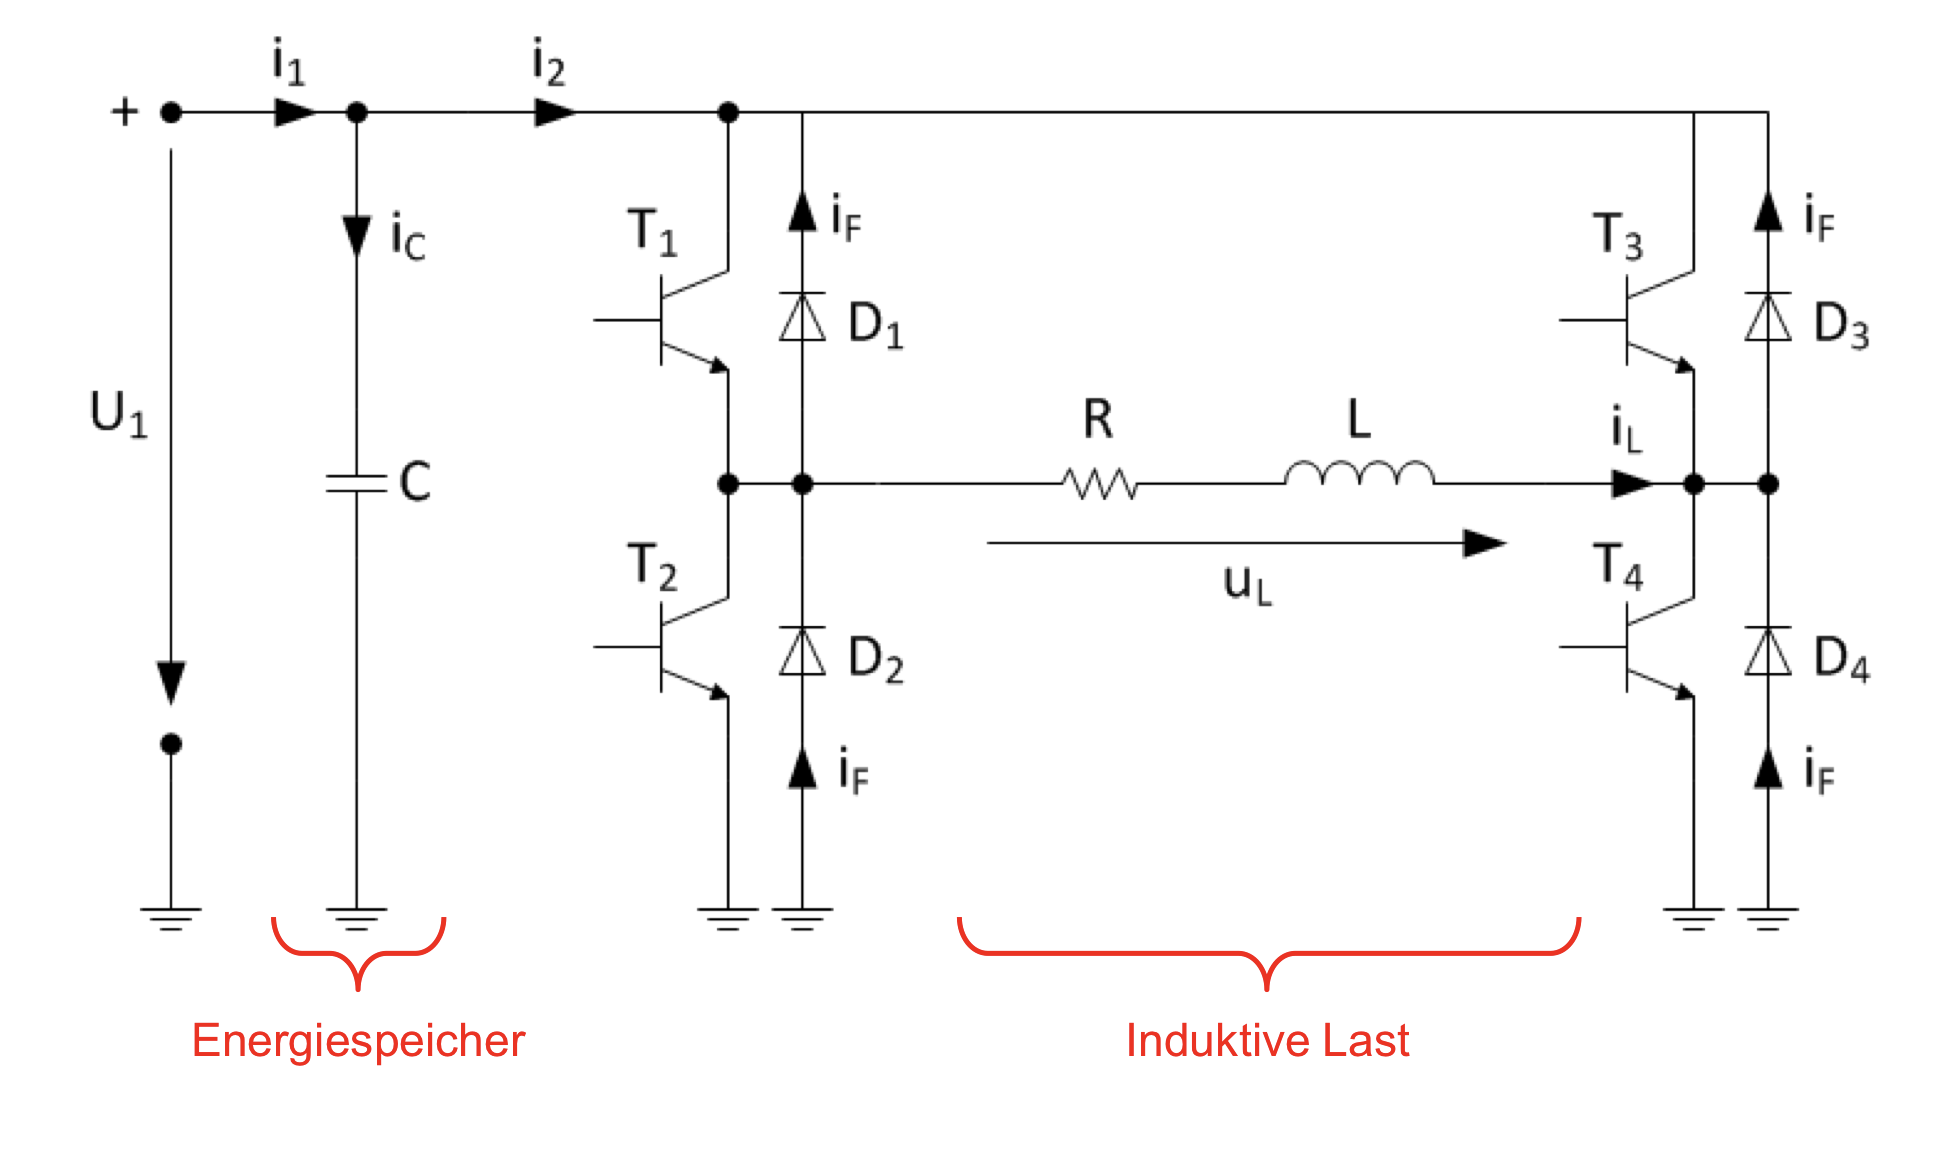
\includegraphics[width=0.85\linewidth]{images/1PWechselrichter.png}
\end{center}

Der einphasige Wechselrichter besteht aus einer H-Brücke mit vier steuerbaren Schaltern.
Durch geeignete Ansteuerung wird am Ausgang abwechselnd $+U_{DC}$ und $-U_{DC}$ erzeugt.
Die Last sieht dadurch eine periodische Wechselspannung.

Zulässige Ausgangsspannungen:
\[
\boxed{u_2(t) \in \{-U_{DC},\; 0,\; +U_{DC}\}}
\]

\subsubsection{Rechteckbetrieb}

Im Grundbetrieb wird mit 50\,\% Tastgrad geschaltet.

\begin{center}
    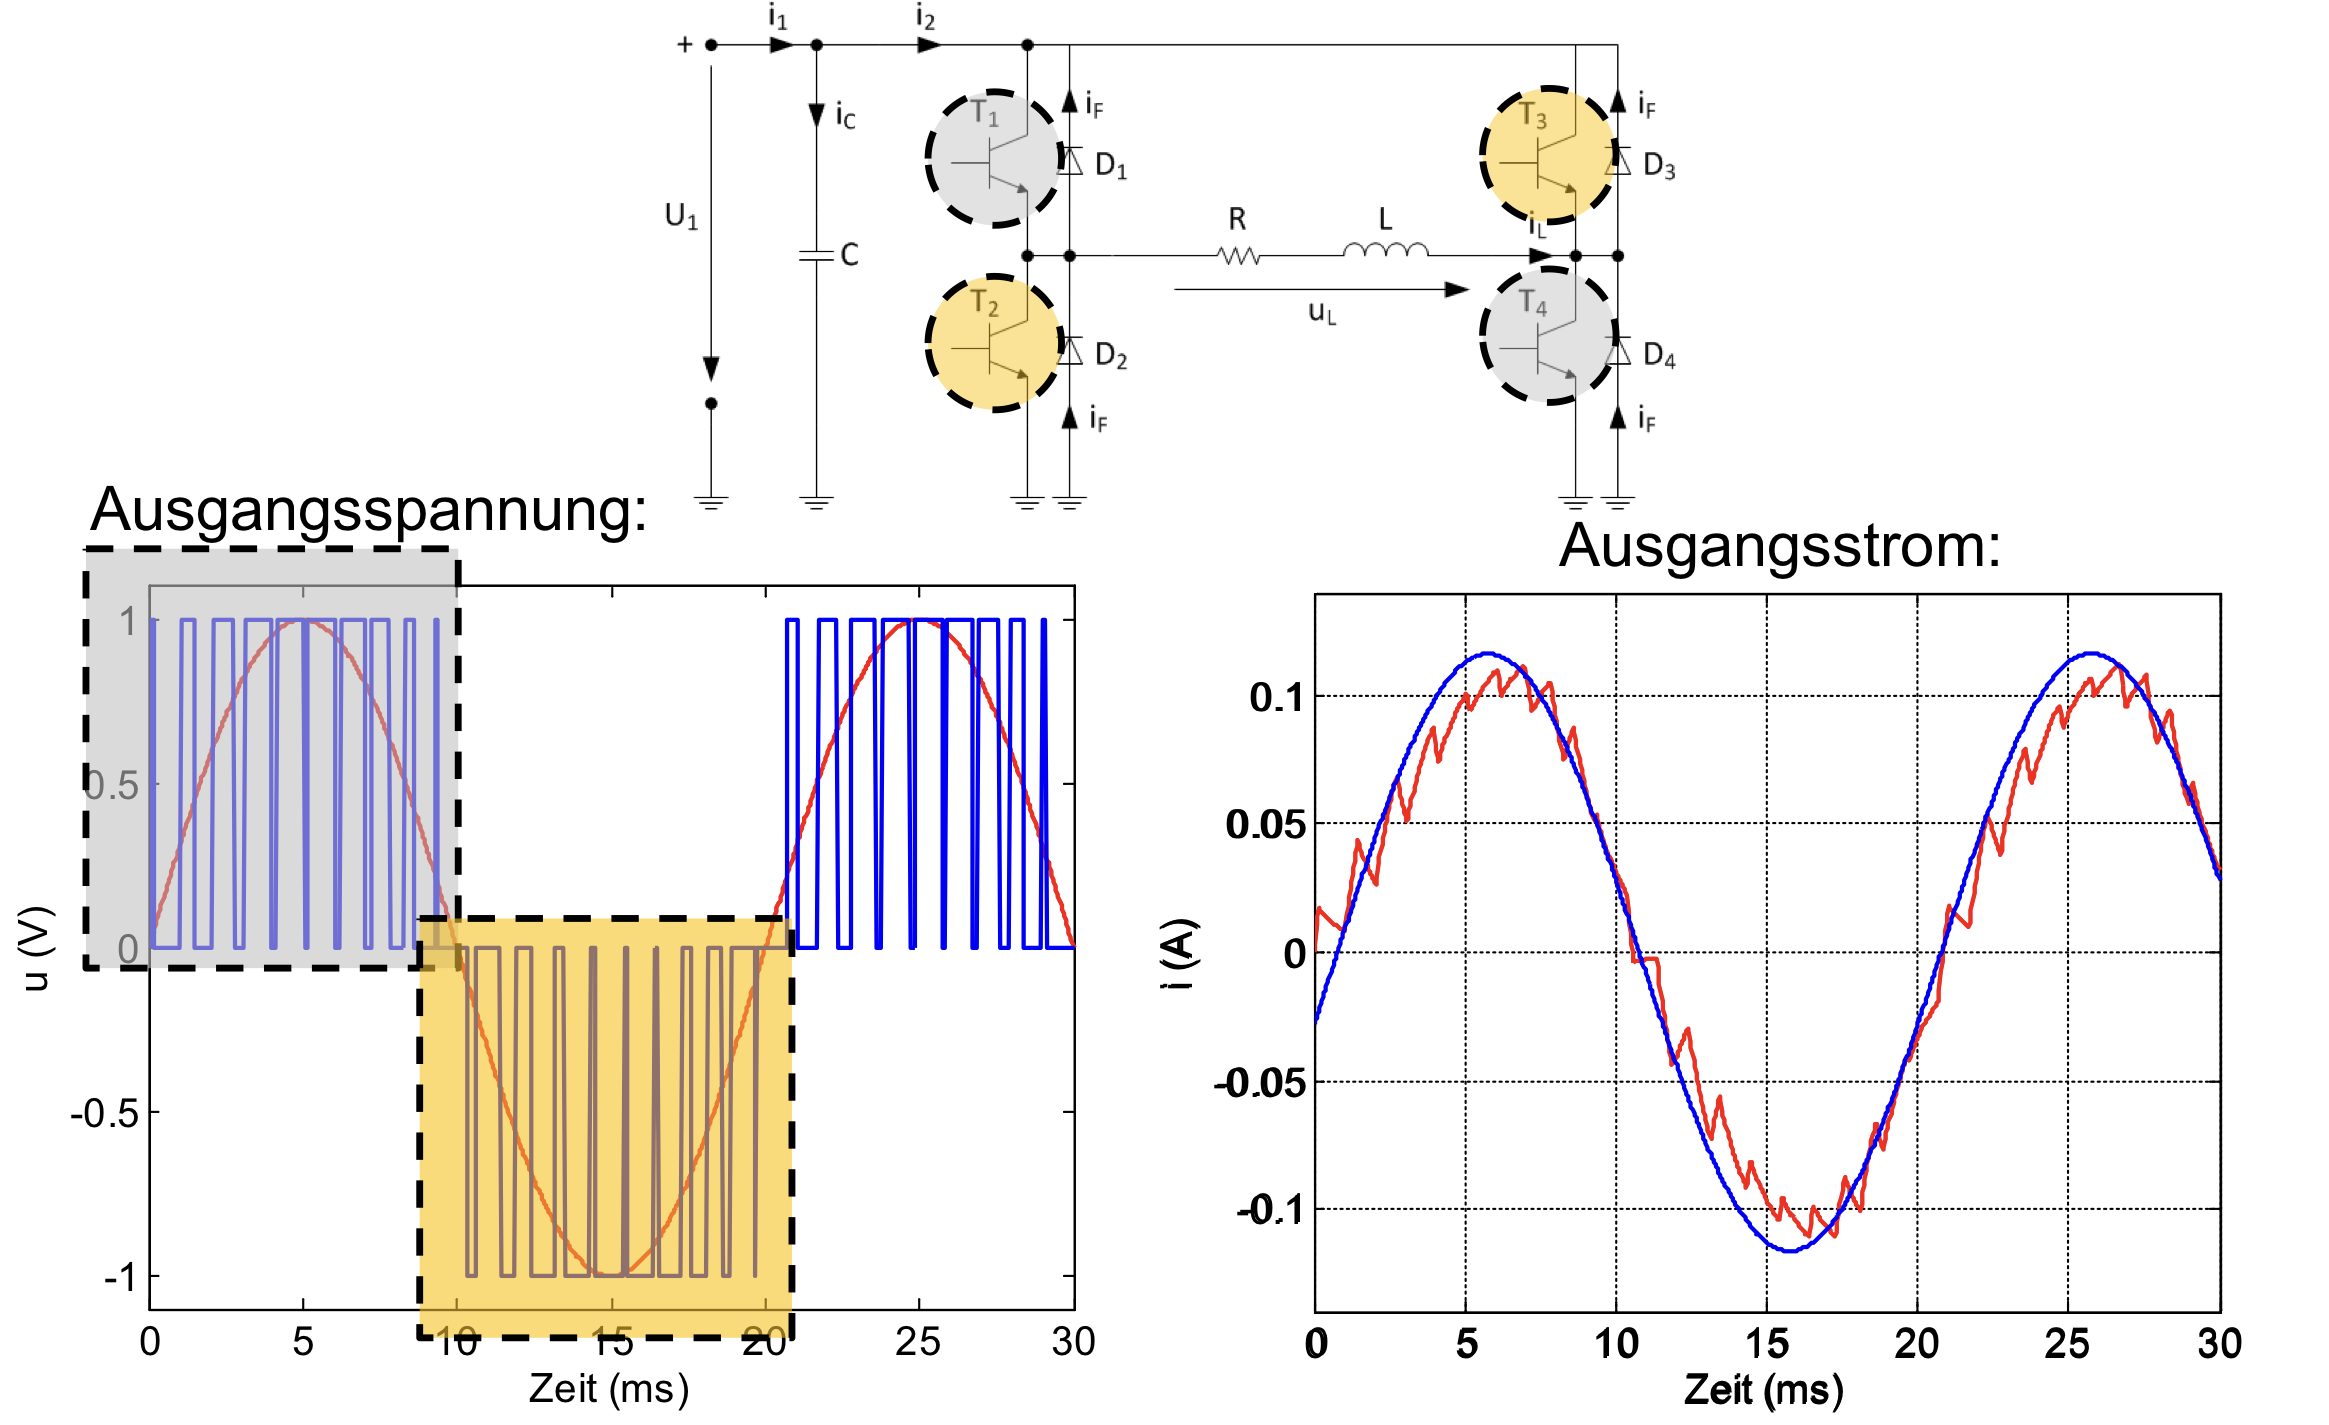
\includegraphics[width=0.85\linewidth]{images/1PWechselrichter_verlauf.png}
\end{center}

Ausgangsspannung:
\[
u_2(t) =
\begin{cases}
+U_{DC}, & 0 < \omega t < \pi \\
- U_{DC}, & \pi < \omega t < 2\pi
\end{cases}
\]

Grundfrequenz:
\[
\boxed{f_1 = \frac{1}{T}}
\]

Effektivwert der Rechteckspannung:
\[
\boxed{U_{\mathrm{RMS}} = U_{DC}}
\]

\paragraph{Erklärung}

Der Rechteckbetrieb ist einfach, liefert jedoch eine stark verzerrte Spannung.
Die Amplitude ist fest durch $U_{DC}$ vorgegeben und nicht steuerbar.
Dieser Betrieb ist nur für einfache Anwendungen geeignet.

\subsubsection{Fourier-Entwicklung}

Fourier-Reihe der Rechteckspannung:
\[
\boxed{
u_2(t) = \frac{4U_{DC}}{\pi}
\left(
\sin\omega t + \frac{1}{3}\sin 3\omega t + \frac{1}{5}\sin 5\omega t + \ldots
\right)
}
\]

Grundschwingungsamplitude:
\[
\boxed{\hat U_1 = \frac{4}{\pi} U_{DC}}
\]

Effektivwert der Grundschwingung:
\[
\boxed{U_{1,\mathrm{RMS}} = \frac{4}{\pi\sqrt{2}} U_{DC}}
\]

\subsubsection{Strom bei R--L-Last}

Lastgleichung:
\[
\boxed{u_2(t) = R i_2(t) + L \frac{di_2(t)}{dt}}
\]

Phasenverschiebung:
\[
\boxed{\tan\varphi = \frac{\omega L}{R}}
\]

Grundstrom:
\[
\boxed{i_{2,1}(t) = \hat I_1 \sin(\omega t - \varphi)}
\]

\paragraph{Erklärung}

Die Induktivität glättet den Strom und verschiebt ihn phasenmäßig nach hinten.
Der Strom enthält deutlich weniger Oberschwingungen als die Spannung.
Freilaufpfade sind zwingend erforderlich.

\subsubsection{PWM-Betrieb (Sinus-PWM)}

Grundschwingungsamplitude:
\[
\boxed{\hat U_1 = m_a \frac{U_{DC}}{2}}, 
\qquad 0 \le m_a \le 1
\]

Effektivwert:
\[
\boxed{U_{1,\mathrm{RMS}} = m_a \frac{U_{DC}}{2\sqrt{2}}}
\]

Grundstrom:
\[
\boxed{I_{1,\mathrm{RMS}} = \frac{U_{1,\mathrm{RMS}}}{\sqrt{R^2 + (\omega L)^2}}}
\]

\paragraph{Erklärung}

Durch PWM kann die Amplitude stufenlos über $m_a$ eingestellt werden.
Die Grundschwingung ist nahezu sinusförmig.
Harmonische liegen um Vielfache der Schaltfrequenz $f_s$.

\subsubsection{Leistungsfluss}

Momentanleistung:
\[
p(t) = u_2(t) i_2(t)
\]

Wirkleistung der Grundschwingung:
\[
\boxed{P = U_{1,\mathrm{RMS}} I_{1,\mathrm{RMS}} \cos\varphi}
\]

Blindleistung:
\[
\boxed{Q = U_{1,\mathrm{RMS}} I_{1,\mathrm{RMS}} \sin\varphi}
\]

\subsubsection{Spezialfälle}

\paragraph{Leerlauf}

\[
\boxed{i_2(t) \approx 0}, 
\qquad
\boxed{P \approx 0}
\]

\paragraph{Kurzschluss}

\[
\boxed{R \approx 0}
\]
\[
\boxed{\frac{di_2}{dt} \approx \frac{u_2(t)}{L}}
\]
\[
\boxed{\left.\frac{di_2}{dt}\right|_{\max} = \frac{U_{DC}}{L}}
\]

% ============================================================
\subsection{Dreiphasiger Wechselrichter}

\subsubsection{Grundschaltung}

\begin{center}
    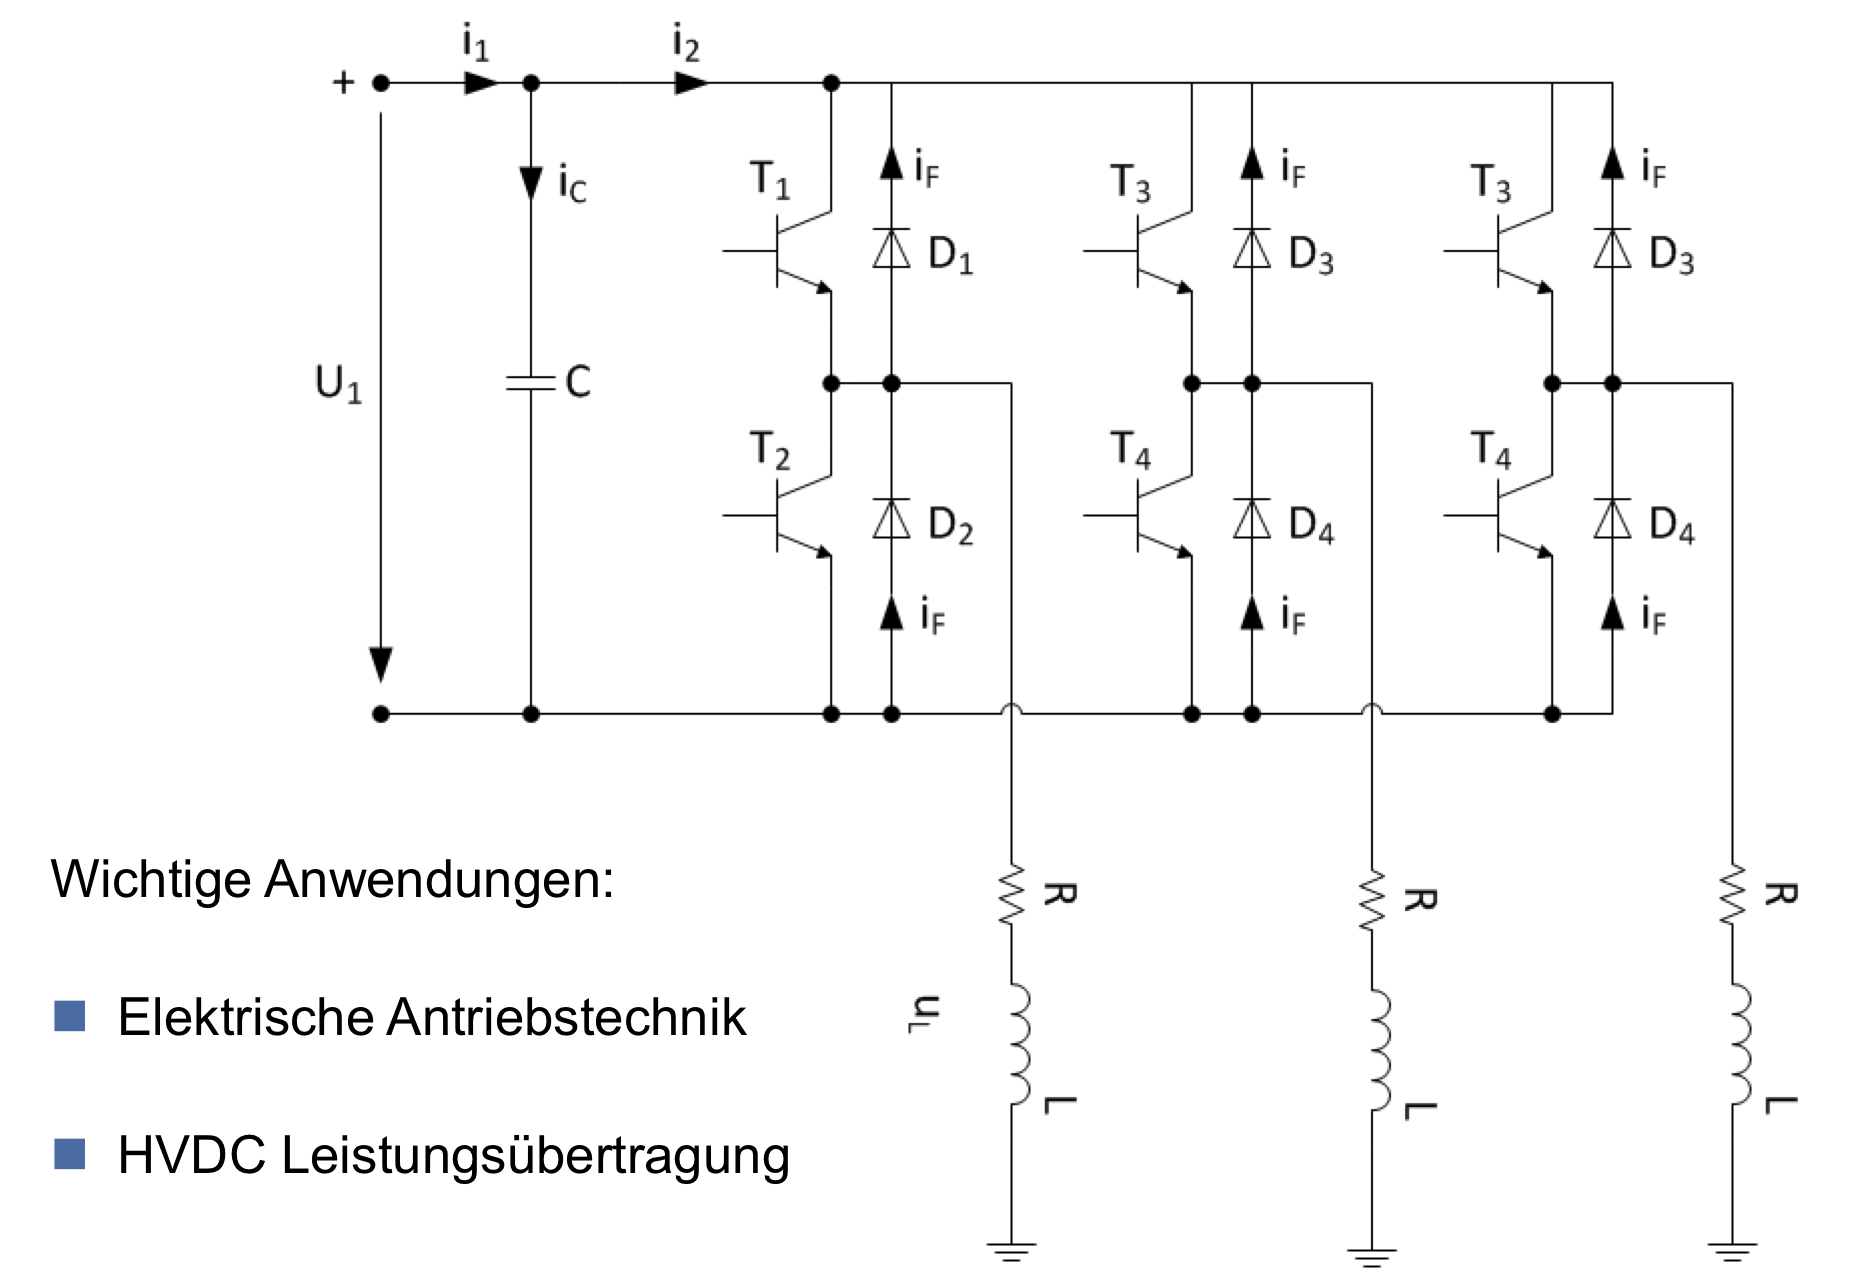
\includegraphics[width=0.85\linewidth]{images/3PWechselrichter.png}
\end{center}

Der dreiphasige Wechselrichter erzeugt drei um $120^\circ$ phasenverschobene Spannungen.
Er liefert bei symmetrischer Last einen nahezu konstanten Leistungsfluss.

Phasenspannungen:
\[
u_a(t),\; u_b(t),\; u_c(t)
\]

Leiterspannungen:
\[
\boxed{u_{ab} = u_a - u_b,\quad u_{bc} = u_b - u_c,\quad u_{ca} = u_c - u_a}
\]

\subsubsection{Grundschwingung}

Phasengrundspannung bei PWM:
\[
\boxed{U_{a,1} = \frac{m_a}{2} U_{DC}}
\]

Leitergrundspannung:
\[
\boxed{U_{LL,1} = \sqrt{3}\, U_{a,1}}
\]

\subsubsection{R--L-Last pro Phase}

Für jede Phase $k \in \{a,b,c\}$:
\[
\boxed{u_k(t) = R i_k(t) + L \frac{di_k}{dt}}
\]

Zeitkonstante:
\[
\boxed{\tau = \frac{L}{R}}
\]

Phasenströme:
\[
i_a(t) = \hat i \sin(\omega t - \varphi)
\]
\[
i_b(t) = \hat i \sin(\omega t - \varphi - \tfrac{2\pi}{3})
\]
\[
i_c(t) = \hat i \sin(\omega t - \varphi + \tfrac{2\pi}{3})
\]

\subsubsection{Leistung im symmetrischen Betrieb}

Mit Phasengrössen:
\[
\boxed{P = 3 U_{\mathrm{ph}} I_{\mathrm{ph}} \cos\varphi}
\]
\[
\boxed{Q = 3 U_{\mathrm{ph}} I_{\mathrm{ph}} \sin\varphi}
\]
\[
\boxed{S = 3 U_{\mathrm{ph}} I_{\mathrm{ph}}}
\]

Mit Leiterspannung:
\[
\boxed{P = \sqrt{3}\, U_{LL} I_L \cos\varphi}
\]

\paragraph{Erklärung}

Der dreiphasige Wechselrichter liefert bei symmetrischer Last einen konstanten Leistungsfluss.
Die Ströme sind sinusförmig und um $120^\circ$ verschoben.
Dieser Betrieb ist Standard in elektrischen Antrieben.

% ============================================================
\subsection{Vergleich Einphasig -- Dreiphasig}

\begin{center}
\begin{tabular}{l|c|c}
 & Einphasig & Dreiphasig \\ \hline
Phasen & 1 & 3 \\
Leistungsfluss & pulsierend & konstant \\
Oberschwingungen & hoch & geringer \\
Anwendungen & klein & Industrie \\
\end{tabular}
\end{center}

\subsection{Merksätze}

\begin{itemize}
    \item Wechselrichter: DC $\rightarrow$ AC mit steuerbarer Frequenz und Amplitude.
    \item Rechteckbetrieb: einfach, aber stark verzerrt.
    \item PWM: sinusförmige Grundschwingung, Amplitude über $m_a$ steuerbar.
    \item Induktive Last glättet den Strom.
    \item Dreiphasig: konstanter Leistungsfluss, Standard in Antrieben.
\end{itemize}
